\documentclass[beamer,crop,tikz]{standalone}


\usepackage{pgf-umlcd}
\renewcommand{\umlfillcolor}{white} 
\renewcommand{\umldrawcolor}{black} 


\begin{document}
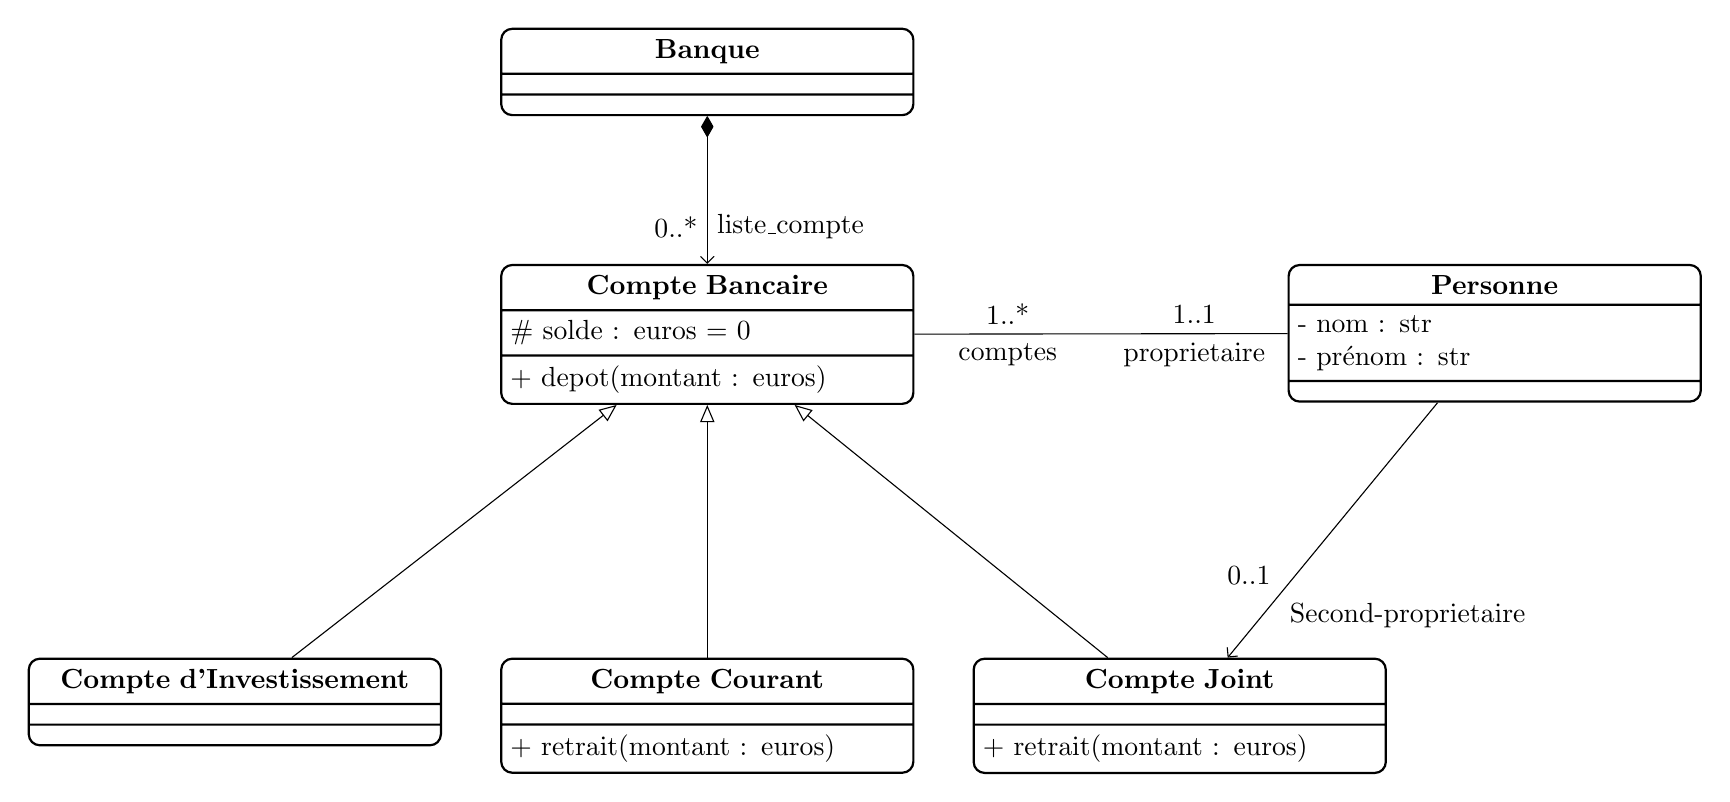
\begin{tikzpicture}
  \begin{class}[rounded corners, thick]{Personne}{10,0}
    \attribute{- nom : str}
    \attribute{- prénom : str}
  \end{class}

  \begin{class}[rounded corners, thick]{Banque}{0,3}
  \end{class}


  \begin{class}[rounded corners, thick]{Compte Bancaire}{0,0}
    \attribute{\# solde : euros = 0}
    \operation{+ depot(montant : euros)}
  \end{class}

  \begin{class}[rounded corners, thick]{Compte Courant}{0,-5}
    \inherit{Compte Bancaire} 
    \operation{+ retrait(montant : euros)}
  \end{class}

  \begin{class}[rounded corners, thick]{Compte Joint}{6,-5}
    \inherit{Compte Bancaire}
    \operation{+ retrait(montant : euros)}
  \end{class}

  \begin{class}[rounded corners, thick]{Compte d'Investissement}{-6,-5}
    \inherit{Compte Bancaire}
  \end{class}

  \composition {Banque}{liste\_compte}{0..*}{Compte Bancaire}
  \association {Personne}{proprietaire}{1..1}{Compte Bancaire}{comptes}{1..*}
  \unidirectionalAssociation {Personne}{Second-proprietaire}{0..1}{Compte Joint}
\end{tikzpicture}
\end{document}
